\documentclass[tikz,border=10mm,12pt]{standalone}
\usepackage{tikz}
\usepackage{pgfplots}
\usepackage{geometry}
\usetikzlibrary{shapes.geometric, arrows, calc, angles, positioning}


% define tikz nodes
\tikzstyle{table} = [rectangle, text centered, minimum width=3cm,
	minimum height=4.5cm, draw=black, fill=black!10]
\tikzstyle{kitchen} = [rectangle, text centered, draw=black, 
minimum width=2cm, minimum height=8cm, fill=black!10]


% define tikz arrows
\tikzstyle{arrow} = [<->, >=stealth, thick]
\tikzstyle{arrow-r} = [<->, >=stealth, thick]

% define environment for legend
\newenvironment{legend}[1][]{
	\begingroup
	\csname pgfplots@init@cleared@structures\endcsname
	\pgfplotsset{#1}}
{\csname pgfplots@createlegend\endcsname
	\endgroup
}

% definition to insert numbers
\pgfkeys{/pgfplots/letter in legend/.style={%
		/pgfplots/legend image code/.code={%
			\node [draw=black, circle, fill=blue!10, inner sep=0.5pt] at (0.295,-0.0225){#1};
		},%
	},
}

% make legend available
\def\addlegendimage{\csname pgfplots@addlegendimage\endcsname}

\begin{document}
	

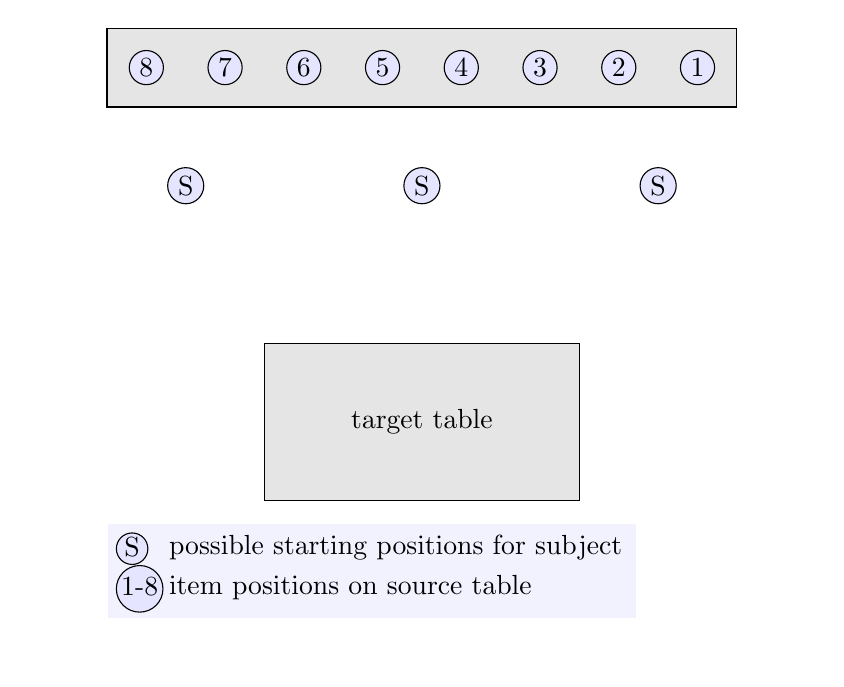
\begin{tikzpicture}
	% set up grid
	\draw[step=9.0, white] (0,0) grid (10,8);

	% set up nodes
	\node (start-table) [rectangle, minimum width=8cm, minimum height=1cm, draw=black, fill=black!10] at (5,7.5) {};
	
	\node (8) [circle, draw=black, inner sep=1.5pt, minimum size=3pt, fill=blue!10] at (1.5,7.5) {8};
	\node (7) [circle, draw=black, inner sep=1.5pt, minimum size=3pt, fill=blue!10] at (2.5,7.5) {7};
	\node (6) [circle, draw=black, inner sep=1.5pt, minimum size=3pt, fill=blue!10] at (3.5,7.5) {6};
	\node (5) [circle, draw=black, inner sep=1.5pt, minimum size=3pt, fill=blue!10] at (4.5,7.5) {5};
	\node (4) [circle, draw=black, inner sep=1.5pt, minimum size=3pt, fill=blue!10] at (5.5,7.5) {4};
	\node (3) [circle, draw=black, inner sep=1.5pt, minimum size=3pt, fill=blue!10] at (6.5,7.5) {3};
	\node (2) [circle, draw=black, inner sep=1.5pt, minimum size=3pt, fill=blue!10] at (7.5,7.5) {2};
	\node (1) [circle, draw=black, inner sep=1.5pt, minimum size=3pt, fill=blue!10] at (8.5,7.5) {1};
	
	\node (table) [rectangle, minimum width=4cm, minimum height=2cm, draw=black, fill=black!10] at (5,3) {};
	
	\node (S) [circle, draw=black, inner sep=1.5pt, minimum size=3pt, fill=blue!10] at (5,6) {S};
	\node (S) [circle, draw=black, inner sep=1.5pt, minimum size=3pt, fill=blue!10] at (2,6) {S};
	\node (S) [circle, draw=black, inner sep=1.5pt, minimum size=3pt, fill=blue!10] at (8,6) {S};
	\node (T) [rectangle, inner sep=1.5pt, minimum size=3pt] at (5,3) {target table};
	

	
	% set up legend entries
	\begin{legend}[legend cell align=left,
	legend style={draw=none, fill=blue!5!white}, 
	legend entries={
		possible starting positions for subject,
		item positions on source table}, 
	legend style={at={(1,0.5)}, anchor=south west}]
	\addlegendimage{letter in legend=S, black}
	\addlegendimage{letter in legend=1-8, black}
	\end{legend}

\end{tikzpicture}


\end{document}